% Uncomment for shell escape
% \RequirePackage{shellesc}

\documentclass{article}

% Font
\usepackage{mlmodern}

% Margins
\usepackage[margin=1in]{geometry}

% Math symbols, proof environments
\usepackage{amsmath, amsthm, amssymb}

% Use this package for matrices
\usepackage{array}

% Images and positioning
\usepackage{graphicx, float, tikz}

% Trees
\usepackage{forest}

% Plots
\usepackage{pgfplots}

\usepackage{xcolor}

\usepackage{parskip}
\usepackage[T1]{fontenc}

% My definitions
\usepackage{mathdefs}

\title{Math 168 Homework 7}

\author{Jason Cheng}

\date{\today}

\begin{document}

\maketitle

\subsection*{Exercise 1}

\begin{enumerate}
  \item[(a)]
  The network represents friendships at a karate club. The reason why it is
  interesting and important is because its members are almost perfectly split
  into two factions, and it illustrates the power of the community detection
  algorithm since the algorithm only incorrectly assigns one member.

  \item[(b)]
  Graphs

  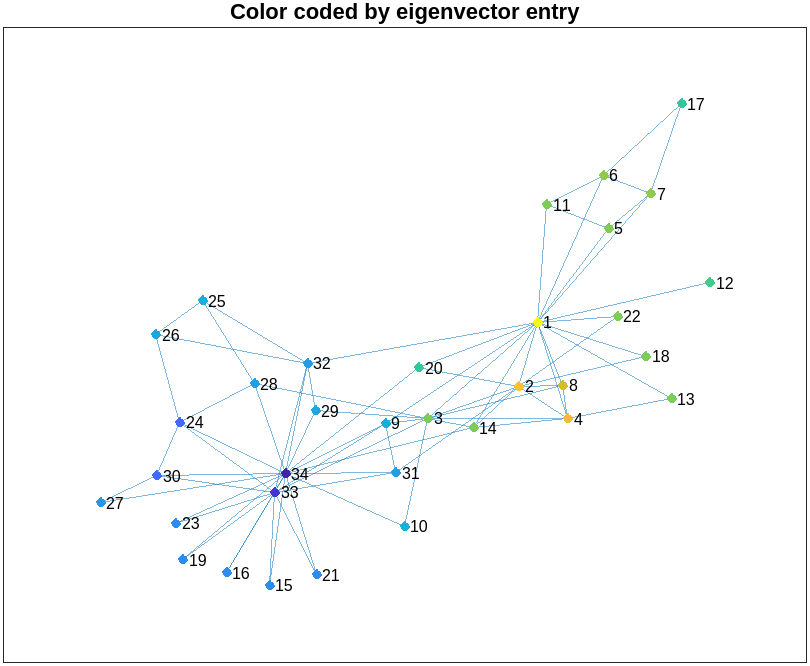
\includegraphics{color-coded.png}

  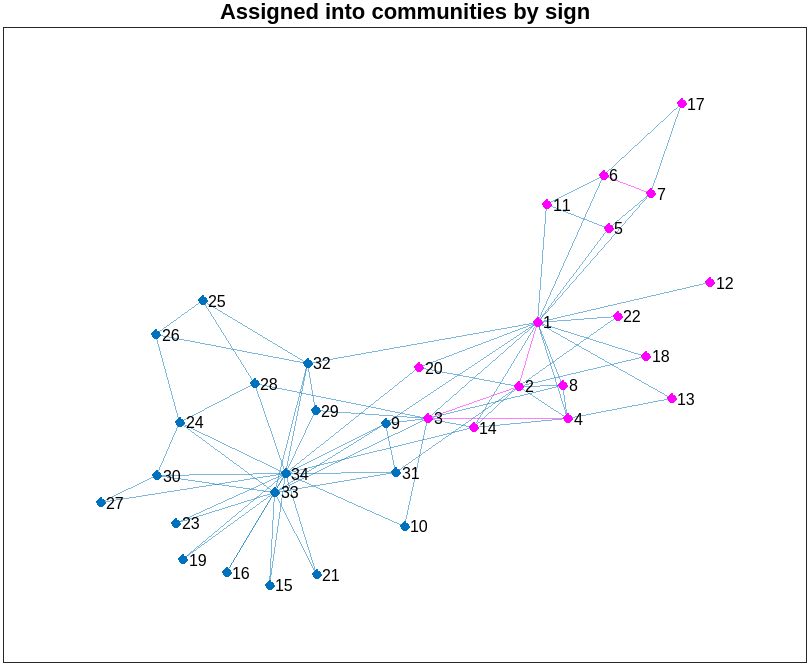
\includegraphics{assigned.png}

  \item[(c)]
  Output:
  \begin{verbatim}
Number of clusters: 1, modularity: -0.000000
Number of clusters: 2, modularity: 0.313281
Number of clusters: 3, modularity: 0.399080
Number of clusters: 4, modularity: 0.419790
Number of clusters: 8, modularity: 0.282873
  \end{verbatim}

  It seems that the modularity is maximized at 4 clusters.

\end{enumerate}

\newpage

\subsection*{Midterm corrections}

1a.

\begin{gather*}
  g_0'(z) = p(1) + p(2) z + p(3) z^2 + \dotsb \\
  g_0'(z) = 1 + \frac{1}{2 - z} \\
  g_0'(1) = p(1) = \boxed{3/2}
\end{gather*}

3c.

\begin{gather*}
  \frac{24(c - 1)}{c / 2 - 1}
\end{gather*}

\newpage

\end{document}
